% ==============================================================================
% intro_stata_basics.tex -- the classroom deck: a short first block on what
% Stata is, then eleven tasks done together in a blank do-file.
% Theme "The Prompt". Compile twice with pdflatex; img/stata_window.png is the
% annotated screenshot on slide 6 (a drawn fallback is used if it is missing).
% ==============================================================================
\documentclass[aspectratio=169,11pt]{beamer}
\usetheme{default}\usecolortheme{default}\usefonttheme{professionalfonts}
\setbeamertemplate{navigation symbols}{}
\usepackage[T1]{fontenc}\usepackage{lmodern}\usepackage[sfdefault]{roboto}
\usepackage{graphicx}\usepackage{tikz}\usetikzlibrary{arrows.meta}\usepackage{ragged2e}\usepackage{array}
\definecolor{PromptMaroon}{HTML}{8C2F39}\definecolor{SlateTeal}{HTML}{3E6B74}
\definecolor{Ink}{HTML}{22303F}\definecolor{WarmGray}{HTML}{6B6560}
\definecolor{MutedOnInk}{HTML}{9AA5B1}\definecolor{Paper}{HTML}{FAF8F3}
\definecolor{PaperDark}{HTML}{EFE9DE}\definecolor{PaperSoft}{HTML}{ECE7DC}
\definecolor{Amber}{HTML}{C98A2D}\definecolor{SoftBlue}{HTML}{7A9CC6}
\definecolor{Forest}{HTML}{2F6B4F}
\setbeamercolor{background canvas}{bg=Paper}\setbeamercolor{normal text}{fg=Ink}
\setbeamercolor{frametitle}{fg=Ink}\setbeamerfont{frametitle}{series=\bfseries,size=\Large}
\setbeamertemplate{frametitle}{\vspace*{0.55cm}{\ttfamily\bfseries\color{PromptMaroon}.\hspace{0.45em}}%
  {\usebeamerfont{frametitle}\usebeamercolor[fg]{frametitle}\insertframetitle}}
\setbeamertemplate{footline}{\hfill{\color{WarmGray}\scriptsize\insertframenumber}\hspace*{3mm}\vspace*{2mm}}
\tikzset{
  win/.style={draw=WarmGray, thick, fill=PaperDark, align=center, inner sep=0pt},
  winlab/.style={font=\ttfamily\bfseries, text=Ink},
  windesc/.style={font=\scriptsize, text=WarmGray},
  flowbox/.style={draw=Ink, thick, fill=PaperDark, align=center, minimum width=3.8cm, minimum height=2.2cm, inner sep=2pt},
  statabox/.style={draw=PromptMaroon, very thick, fill=PromptMaroon!12!Paper, align=center, minimum width=2.2cm, minimum height=2.2cm},
  flowarrow/.style={-{Stealth[length=3mm]}, very thick, draw=Ink},
}
% one command per row: mono command, then what it does, in the deck's voice
\newenvironment{cmds}{\begin{center}\begin{minipage}{0.92\textwidth}\RaggedRight\setlength{\parskip}{0.5em}}{\end{minipage}\end{center}}
\newcommand{\cmd}[2]{{\ttfamily\color{SlateTeal}#1}\hspace{0.6em}{\small\color{Ink}#2}\par}
\newcommand{\ask}[1]{\vspace*{0.15cm}{\small\itshape\color{WarmGray}the email asks: #1}\par\vspace{0.35em}}
\newcommand{\yourturn}[1]{\vspace{0.5em}\begin{center}{\color{PromptMaroon}\small #1}\end{center}}
\newcommand{\answer}[1]{\begin{center}\begin{minipage}{0.92\textwidth}\RaggedRight\setlength{\fboxsep}{6pt}\colorbox{PaperDark}{\begin{minipage}{\dimexpr\textwidth-12pt}\RaggedRight\small #1\end{minipage}}\end{minipage}\end{center}}
\begin{document}

% 1 --------------------------------------------------------------------- title
{\setbeamercolor{background canvas}{bg=Ink}%
\begin{frame}[plain]
  \centering\vfill
  {\ttfamily\bfseries\color{Amber}\Large .\hspace{0.45em}}{\color{white}\Huge\bfseries Intro to Stata}\\[1.0em]
  {\color{PaperSoft}\large A hands-on session}\\[0.35em]
  {\color{MutedOnInk}University of Groningen}\\[2.2em]
  {\color{PaperSoft}Ade Febriady}\\[0.35em]
  {\color{MutedOnInk}\small Friday 11 September 2026 \,\textperiodcentered\, 11:00--12:45}
  \vfill
\end{frame}}

% 2 ------------------------------------------------------ hook: the email
\begin{frame}{An email you will get}
  \centering\vspace*{0.15cm}
  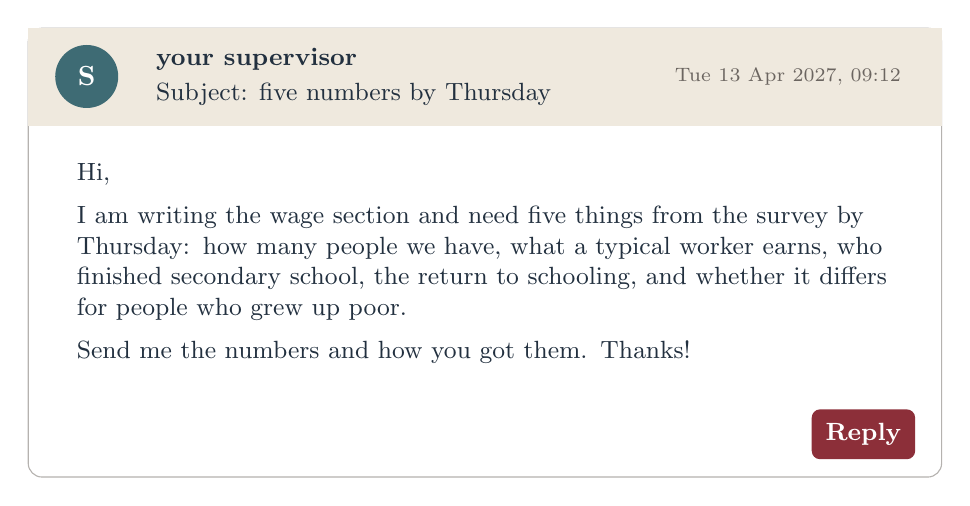
\begin{tikzpicture}
    \node[draw=WarmGray!50, fill=white, rounded corners=5pt, inner sep=0, minimum width=11.6cm, minimum height=5.7cm] (card) at (0,0) {};
    \fill[PaperDark] ([yshift=-1.25cm]card.north west) rectangle (card.north east);
    \node[circle, fill=SlateTeal, text=white, font=\bfseries, minimum size=0.8cm, inner sep=0] (av) at ([xshift=0.75cm, yshift=-0.62cm]card.north west) {S};
    \node[anchor=west, font=\small\bfseries, text=Ink] at ([xshift=0.35cm, yshift=0.22cm]av.east) {your supervisor};
    \node[anchor=west, font=\small, text=Ink] at ([xshift=0.35cm, yshift=-0.22cm]av.east) {Subject: five numbers by Thursday};
    \node[anchor=east, font=\scriptsize, text=WarmGray] at ([xshift=-0.4cm, yshift=-0.62cm]card.north east) {Tue 13 Apr 2027, 09:12};
    \node[anchor=north west, text width=10.6cm, font=\small, text=Ink, align=left] at ([xshift=0.5cm, yshift=-1.6cm]card.north west) {Hi,\\[0.5em]
      I am writing the wage section and need five things from the survey by Thursday: how many people we have, what a typical worker earns, who finished secondary school, the return to schooling, and whether it differs for people who grew up poor.\\[0.5em]
      Send me the numbers and how you got them. Thanks!};
    \node[fill=PromptMaroon, text=white, rounded corners=3pt, font=\small\bfseries, inner sep=5pt] at ([xshift=-1.0cm, yshift=0.55cm]card.south east) {Reply};
  \end{tikzpicture}
  \vspace*{0.3cm}

  {\color{PromptMaroon}\large by 12:45 you can answer it}
\end{frame}

% ------------------------------------------------------------------ why Stata
\begin{frame}{Why Stata}
  \vspace*{0.6cm}
  \begin{columns}[T]
    \column{0.32\textwidth}\centering
      {\ttfamily\color{SlateTeal}journals}\\[0.5em]
      {\fontsize{34}{36}\selectfont\bfseries\color{PromptMaroon}\vphantom{jl}73\%}\\[0.5em]
      {\small of the code packages in the AEA archive use Stata\textsuperscript{1}}
    \column{0.32\textwidth}\centering
      {\ttfamily\color{SlateTeal}surveys}\\[0.5em]
      {\fontsize{34}{36}\selectfont\bfseries\color{PromptMaroon}\vphantom{jl}.dta}\\[0.5em]
      {\small LSMS and DHS are available as Stata files\textsuperscript{2}}
    \column{0.32\textwidth}\centering
      {\ttfamily\color{SlateTeal}jobs}\\[0.5em]
      {\fontsize{34}{36}\selectfont\bfseries\color{PromptMaroon}\vphantom{jl}.do}\\[0.5em]
      {\small employers, e.g. the World Bank, set Stata tests and ask to see your do-file\textsuperscript{3}}
  \end{columns}
  \vspace*{0.6cm}\centering
  {\color{WarmGray}\small the habit, a script and a log, moves to R or Python unchanged}
  \vfill
  \begin{flushleft}
  {\color{WarmGray}\scriptsize \textsuperscript{1}\,Vilhuber, Turitto and Welch (2020), \emph{AEA Papers and Proceedings} 110: 764--775, corrigendum of 4 Aug 2020.\quad
  \textsuperscript{2}\,DHS Program, File Formats; World Bank Microdata Library.\quad \textsuperscript{3}\,Personal experience, World Bank consultancy recruitment.}
  \end{flushleft}
\end{frame}

% 3 ---------------------------------------------------------- three ways (her 6)
\begin{frame}{You talk to Stata in commands}
  \vfill\centering
  {\color{WarmGray}three ways to give one, and today is the third}\\[1.4em]
  \begin{tabular}{@{}l>{\RaggedRight\arraybackslash}p{8.4cm}@{}}
    {\ttfamily\color{WarmGray}menus} & click through the drop-down menus. Stata prints the command each click ran, so you can copy it\\[0.6em]
    {\ttfamily\color{WarmGray}Command window} & type one command, press Enter, read the answer\\[0.6em]
    {\ttfamily\bfseries\color{PromptMaroon}do-file} & write the commands in a text file, run the file. Your work is saved, repeatable, and can be checked by someone else\\
  \end{tabular}
  \vfill
\end{frame}

% 3 --------------------------------------------------------- getting Stata (her 3)
\begin{frame}{The university gives you Stata two ways}
  \vspace*{0.9cm}
  \begin{columns}[T]
    \begin{column}{0.44\textwidth}\centering
      {\ttfamily\bfseries\color{SlateTeal}uwp.rug.nl}\\[0.6em]
      {\small the university's virtual workplace.\\ sign in with your student account}
    \end{column}
    \begin{column}{0.44\textwidth}\centering
      {\ttfamily\bfseries\color{SlateTeal}IRIS}\\[0.6em]
      {\small download and install it\\ on your own machine, for later}
    \end{column}
  \end{columns}
\end{frame}

% 4 ------------------------------------------------------- four windows (her 4-5)
\IfFileExists{img/stata_window.png}{%
\begin{frame}{Stata is four windows and one editor}
  \centering\vspace*{0.05cm}
  \begin{tikzpicture}
    \node[anchor=south west, inner sep=0] (img) at (0,0) {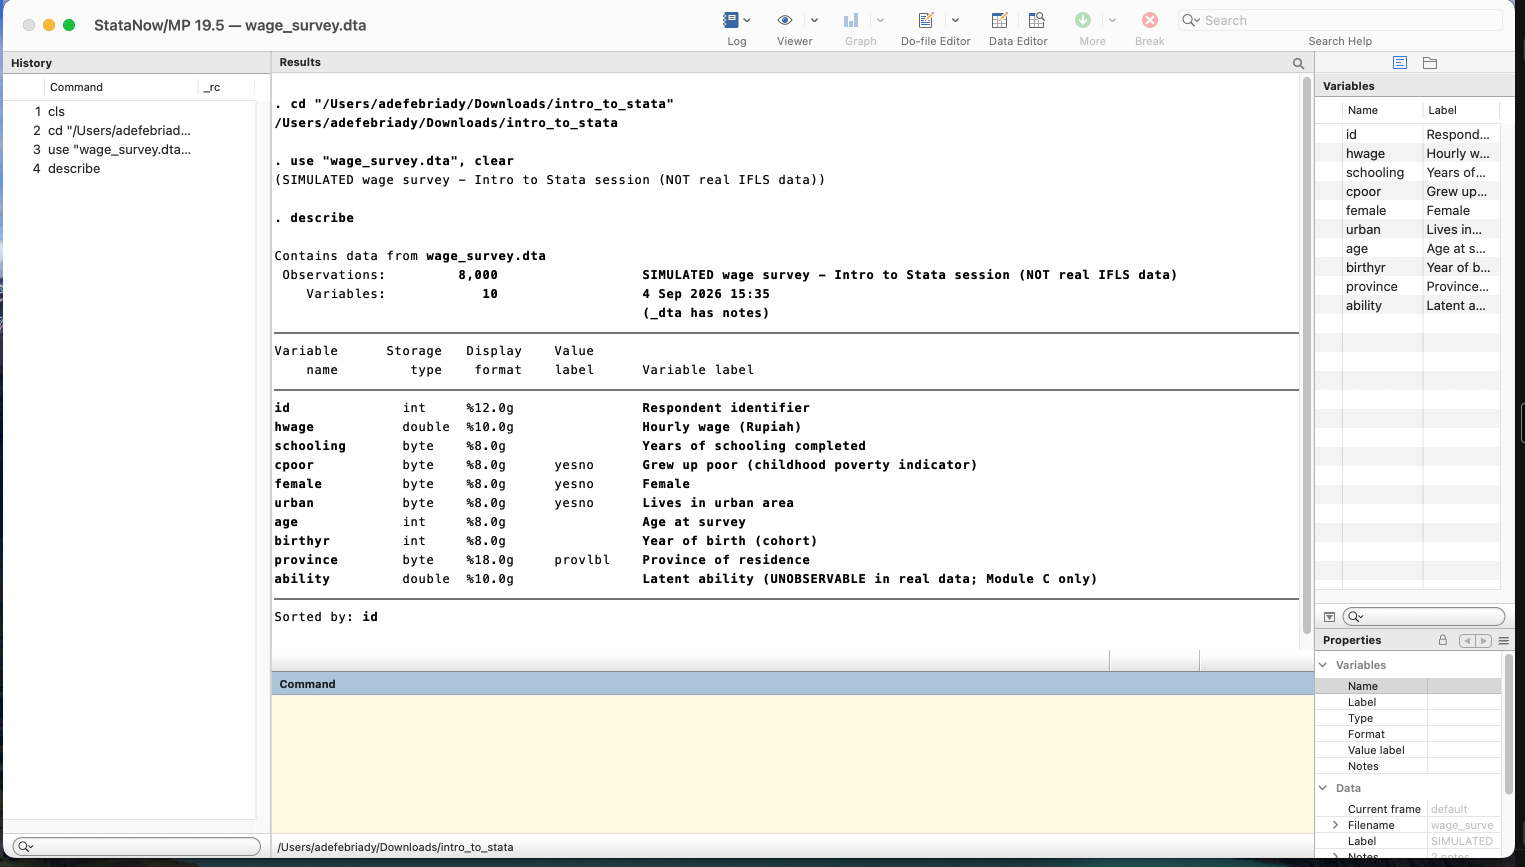
\includegraphics[width=11.0cm]{img/stata_window.png}};
    \begin{scope}[x={(img.south east)}, y={(img.north west)}]
      \node[fill=PromptMaroon, text=white, font=\ttfamily\bfseries\small, inner sep=3pt] at (0.085, 0.578) {history};
      \node[fill=PromptMaroon, text=white, font=\ttfamily\bfseries\small, inner sep=3pt] at (0.52, 0.578) {results};
      \node[fill=PromptMaroon, text=white, font=\ttfamily\bfseries\small, inner sep=3pt] at (0.52, 0.128) {command};
      \node[fill=PromptMaroon, text=white, font=\ttfamily\bfseries\small, inner sep=3pt] at (0.925, 0.578) {variables};
      \node[fill=WarmGray, text=white, font=\ttfamily\small, inner sep=3pt] at (0.925, 0.14) {properties: ignore};
      \node[fill=Amber, text=Ink, font=\ttfamily\bfseries\small, inner sep=3pt] (ed) at (0.613, 0.87) {Do-file Editor};
      \draw[-{Stealth[length=2mm]}, Amber, very thick] (ed.north) -- (0.613, 0.955);
    \end{scope}
  \end{tikzpicture}

  {\color{WarmGray}\small the windows are Stata talking to you; the editor, one click away, is you talking back.\\ On the lab's Windows machines the boxes sit in a different order; the four are the same}
\end{frame}
}{%
\begin{frame}{Stata is four windows and one editor}
  \centering\vspace*{0.25cm}
  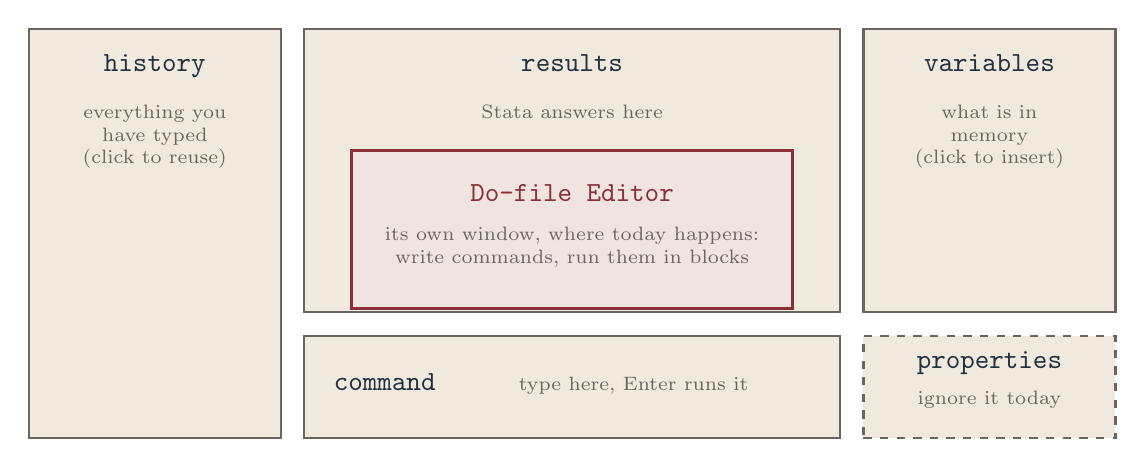
\begin{tikzpicture}
    \node[win, minimum width=3.2cm, minimum height=5.2cm] at (1.6, 2.6) {};
    \node[winlab, anchor=north] at (1.6, 5.0) {history};
    \node[windesc, anchor=north, text width=2.8cm, align=center] at (1.6, 4.35) {everything you\\ have typed\\ (click to reuse)};
    \node[win, minimum width=6.8cm, minimum height=3.6cm] at (6.9, 3.4) {};
    \node[winlab, anchor=north] at (6.9, 5.0) {results};
    \node[windesc, anchor=north] at (6.9, 4.35) {Stata answers here};
    \node[win, minimum width=6.8cm, minimum height=1.3cm] at (6.9, 0.65) {};
    \node[winlab, anchor=base west] at (3.75, 0.60) {command};
    \node[windesc, anchor=base west] at (6.1, 0.60) {type here, Enter runs it};
    \node[win, minimum width=3.2cm, minimum height=3.6cm] at (12.2, 3.4) {};
    \node[winlab, anchor=north] at (12.2, 5.0) {variables};
    \node[windesc, anchor=north, text width=2.8cm, align=center] at (12.2, 4.35) {what is in\\ memory\\ (click to insert)};
    \node[win, dashed, minimum width=3.2cm, minimum height=1.3cm] at (12.2, 0.65) {};
    \node[winlab, anchor=north] at (12.2, 1.22) {properties};
    \node[windesc, anchor=north] at (12.2, 0.72) {ignore it today};
    \node[draw=PromptMaroon, very thick, fill=PromptMaroon!10!Paper, minimum width=5.6cm, minimum height=2.0cm, align=center] at (6.9, 2.65) {};
    \node[winlab, text=PromptMaroon, anchor=north] at (6.9, 3.35) {Do-file Editor};
    \node[windesc, anchor=north, text width=5.4cm, align=center] at (6.9, 2.80) {its own window, where today happens:\\ write commands, run them in blocks};
  \end{tikzpicture}
  \vspace*{0.35cm}

  {\color{WarmGray}\small the four windows are Stata talking to you; the editor is you talking back}
\end{frame}
}


% --------------------------------------------------- click once, copy the command
\begin{frame}{Click once, then copy what Stata typed}
  \vspace*{0.5cm}
  \begin{cmds}
    \cmd{File > Open}{opens the data by clicking. Look at the Results window: Stata prints the command it just ran}
    \cmd{use "wage\_survey.dta", clear}{that printed line. Copy it into your do-file, and it is yours forever}
    \cmd{Statistics > Summaries > Summary statistics}{the same trick for any command you do not know yet}
  \end{cmds}
  \vspace*{0.9cm}\centering
  {\color{WarmGray}\small the menus are a way to find a command; the do-file is where you keep it}
\end{frame}

% 5 ------------------------------------------------------- do-file, log (her 9-10)
\begin{frame}{You write the do-file; Stata writes the log}
  \centering\vspace*{0.9cm}
  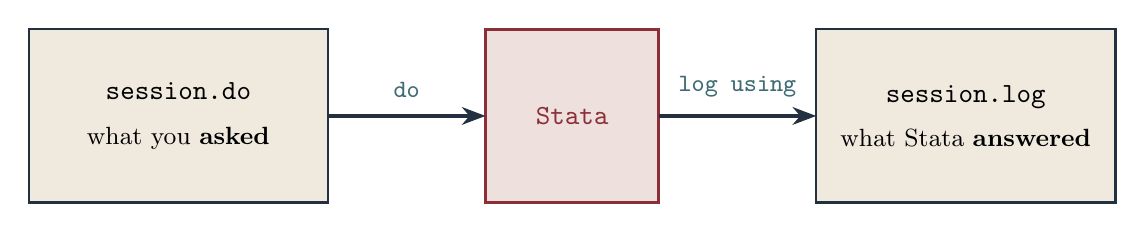
\begin{tikzpicture}
    \node[flowbox] at (1.9, 0) {{\ttfamily\bfseries session.do}\\[0.4em]\small what you \textbf{asked}};
    \node[statabox] at (6.9, 0) {{\ttfamily\bfseries\color{PromptMaroon}Stata}};
    \node[flowbox] at (11.9, 0) {{\ttfamily\bfseries session.log}\\[0.4em]\small what Stata \textbf{answered}};
    \draw[flowarrow] (3.8, 0) -- (5.8, 0) node[midway, above, yshift=1mm, font=\ttfamily\small, text=SlateTeal] {do};
    \draw[flowarrow] (8.0, 0) -- (10.0, 0) node[midway, above, yshift=1mm, font=\ttfamily\small, text=SlateTeal] {log using};
  \end{tikzpicture}
  \vspace*{1.1cm}

  {\color{WarmGray}keep both; next week's you can re-read today}
\end{frame}

% ------------------------------------------------------ anatomy of a do-file
\begin{frame}{The anatomy of a do-file}
  \vspace*{0.35cm}
  \begin{cmds}
    \cmd{* a note for people}{Stata skips everything after a star}
    \cmd{summarize \ \ // a note at the end of a line}{two slashes do the same, after a command}
    \cmd{/* a longer note, over several lines */}{for a paragraph}
    \cmd{**\# 3. Look at the data}{a bookmark. The editor lists them, so a long file has a table of contents}
    \cmd{cd "..."}{the first real command: where your folder is}
    \cmd{log using "session.log", replace}{the second: keep a record of everything from here}
  \end{cmds}
  \vspace*{0.5cm}\centering
  {\color{WarmGray}\small notes first, then the two lines every do-file starts with, then the work}
\end{frame}

% --------------------------------------------------------------- file types
\begin{frame}{Four kinds of file}
  \vspace*{0.4cm}
  \begin{cmds}
    \cmd{.dta}{data, in Stata's own format. \texttt{use} opens one, \texttt{save} writes one}
    \cmd{.do}{a do-file: your commands, in order, with your notes. The thing you write today}
    \cmd{.log}{the log: everything Stata printed while the do-file ran. The thing you hand in}
    \cmd{.ado}{a command that somebody wrote in Stata. \texttt{help} shows it like any other; \texttt{ssc install} fetches new ones}
  \end{cmds}
  \vspace*{0.9cm}\centering
  {\color{WarmGray}\small the do-file makes the log from the data. Keep all three together in one folder}
\end{frame}

% 6 ---------------------------------------------------------- what you get (ours)
\begin{frame}{What you get}
  \vspace*{0.4cm}
  \begin{cmds}
    \cmd{wage\_survey.dta}{on Brightspace: the dataset, 8,000 simulated wage workers, made to look like a real Indonesian survey}
    \cmd{exercise.html}{on Brightspace: the tasks we do together, with every answer folded away until you click. Open it now}
    \cmd{session.do}{on Brightspace: the finished do-file, to check your own against afterwards}
  \end{cmds}
  \vspace*{0.9cm}\centering
  {\color{WarmGray}\small nothing to install. save the download in a folder you can find again}
\end{frame}

% 7 ------------------------------------------------------ setup: ten minutes
\begin{frame}{Ten minutes: tell Stata where your folder is}
  \vspace*{0.3cm}
  \begin{cmds}
    \cmd{cd "C:/Users/you/Downloads/intro\_to\_stata"}{your folder, wherever you saved it. Find it once: File > Change Working Directory, pick it, then type \texttt{display c(pwd)} and copy the answer}
    \cmd{capture log close}{closes a log if one is open, and says nothing if not}
    \cmd{log using "session.log", replace}{from here on, everything is written down}
    \cmd{use "wage\_survey.dta", clear}{opens the data; \texttt{clear} drops whatever was in memory first}
  \end{cmds}
  \vspace*{0.6cm}\centering
  {\color{WarmGray}\small the first four lines of your do-file. Type them, run them.}\\[0.3em]
  {\color{PromptMaroon}\small ``file not found'' means the folder line. Raise a hand; that is what the ten minutes are for}
\end{frame}

% 8 ---------------------------------------------------------- the email arrives
\begin{frame}{The email arrives}
  \vspace*{0.2cm}
  \begin{center}
  \begin{minipage}{0.94\textwidth}\RaggedRight\small
    Hi, I am writing the wage section and need five things from the survey by Thursday.\\[0.5em]
    \begin{tabular}{@{}r>{\RaggedRight\arraybackslash}p{11.6cm}@{}}
      {\color{Amber}\ttfamily 1--4} & how many people do we actually have, and what do they look like?\\
      {\color{Amber}\ttfamily 5} & what does a typical worker earn?\\
      {\color{Amber}\ttfamily 6} & what share finished secondary school, and is it lower for people who grew up poor?\\
      {\color{Amber}\ttfamily 7--9} & what is the return to a year of schooling, holding province, gender, age and location fixed?\\
      {\color{Amber}\ttfamily 10} & does that return look different for people who grew up poor?\\
    \end{tabular}\\[0.5em]
    Send me the numbers and how you got them. Thanks!
  \end{minipage}
  \end{center}
  \vspace*{0.3cm}\centering
  {\color{WarmGray}\small eleven tasks, one command or two each. Run it, read it, then we talk}
\end{frame}

% --------------------------------------------------------------------- task 1
\begin{frame}{1. Open the data}
  \ask{how many people do we actually have?}
  \begin{cmds}
    \cmd{use "wage\_survey.dta", clear}{again, from the do-file: a do-file works from the top}
  \end{cmds}
  \yourturn{run it. What did Stata print?}
  \pause
  \answer{One line, the data label. Stata is quiet when things work.}
\end{frame}

% --------------------------------------------------------------------- task 2
\begin{frame}{2. How many people, and what is in the file}
  \ask{how many people do we actually have?}
  \begin{cmds}
    \cmd{describe}{every variable, its label, how many rows}
  \end{cmds}
  \yourturn{how many observations, how many variables?}
  \pause
  \answer{8,000 and 10. ``Actually'' is doing some work in that question.}
\end{frame}

% --------------------------------------------------------------------- task 3
\begin{frame}{3. What do they look like}
  \ask{...and what do they look like?}
  \begin{cmds}
    \cmd{summarize}{mean, min, max, N of every number}
  \end{cmds}
  \yourturn{two numbers in that table should bother you. Which?}
  \pause
  \answer{The maximum age is 320, and schooling has 7,800 answers, not 8,000.\\[0.3em] For the reply: 40 percent women, 55 percent urban, 28 percent grew up poor, mean age 25, mean schooling 10 years.}
\end{frame}

% --------------------------------------------------------------------- task 4
\begin{frame}{4. But first, those ages}
  \ask{how many people do we \emph{actually} have?}
  \begin{cmds}
    \cmd{histogram age}{one crushed bar: a picture shows a wrong value first}
    \cmd{list id age birthyr if age > 100}{the people above 100, with year of birth}
  \end{cmds}
  \yourturn{ten people. What happened to them, and what can you do about it?}
  \pause
  \answer{An extra zero: born 1994, surveyed 2014, so 20, not 200. The file knows the right value, so repair it:\\[0.2em]{\ttfamily\color{SlateTeal}replace age = 2014 - birthyr if age > 100}\\[0.2em] Ten changes; ages run 15 to 35 again.}
\end{frame}

% --------------------------------------------------------------------- task 5
\begin{frame}{5. What does a typical worker earn}
  \ask{what does a typical worker earn?}
  \begin{cmds}
    \cmd{summarize hwage, detail}{one variable, with percentiles}
  \end{cmds}
  \yourturn{mean, median, 25th and 75th percentile. Which one answers the question?}
  \pause
  \answer{Mean 11,218, median 8,571. A few high earners pull the mean up. Report the median, and say so.}
\end{frame}

% --------------------------------------------------------------------- task 6
\begin{frame}{6. Secondary school, by background}
  \ask{what share finished secondary school, and is it lower for people who grew up poor?}
  \begin{cmds}
    \cmd{generate high = schooling >= 12}{a new variable: 1 if the condition holds, 0 if not}
    \cmd{tabulate high, missing}{count each value, and show the missing ones too}
  \end{cmds}
  \yourturn{is the table right?}
  \pause
  \answer{No. 5,220 zeros, 2,780 ones, no missing: the 200 without an answer all became 1. Stata stores missing as larger than any number.}
\end{frame}

\begin{frame}{6, continued: say what you mean}
  \vspace*{0.3cm}
  \begin{cmds}
    \cmd{drop high}{throw the wrong one away}
    \cmd{generate high = schooling >= 12 if !missing(schooling)}{only for people who answered}
    \cmd{tabulate high, missing}{5,220 zeros, 2,580 ones, 200 missing. Right}
    \cmd{tabulate cpoor high, row}{the cross-table, with row percentages}
  \end{cmds}
  \yourturn{read the row percentages}
  \pause
  \answer{38 percent of the never-poor, 21 percent of those who grew up poor.\\[0.3em]{\color{PromptMaroon}every \texttt{>} or \texttt{>=} on a variable that can be missing needs \texttt{\& !missing()}.} In SAS missing is smaller than any number, so there the trap sits in \texttt{<}.}
\end{frame}

% --------------------------------------------------------------------- task 7
\begin{frame}{7. The return to a year of schooling}
  \ask{the return to a year of schooling, holding province, gender, age and location fixed}
  \begin{cmds}
    \cmd{generate lhwage = ln(hwage)}{the log of the wage: a change of 0.01 is about 1 percent}
    \cmd{regress lhwage schooling female urban age i.province}{\texttt{i.province} turns one variable into a dummy per province}
  \end{cmds}
  \yourturn{read two numbers: N, and the coefficient on schooling}
  \pause
  \answer{N 7,800: the 200 without schooling are silently left out. Schooling 0.079: a year of schooling is associated with an 8 percent higher wage.\\[0.3em] Skipped task 4? Then look at the coefficient on age.}
\end{frame}

% --------------------------------------------------------------------- task 8
\begin{frame}{8. Did the model behave \hfill{\small\color{WarmGray}if time allows}}
  \vspace*{0.3cm}
  \begin{cmds}
    \cmd{predict yhat}{the fitted value, from the regression still in memory}
    \cmd{predict uhat, residuals}{actual minus fitted}
    \cmd{summarize yhat uhat}{their means, and their N}
  \end{cmds}
  \yourturn{what is the mean of the residuals, and why?}
  \pause
  \answer{Zero, by construction: OLS picks the coefficients that make the residuals average zero. Both N are 7,800.}
\end{frame}

% --------------------------------------------------------------------- task 9
\begin{frame}{9. One number for the relationship \hfill{\small\color{WarmGray}if time allows}}
  \vspace*{0.3cm}
  \begin{cmds}
    \cmd{correlate hwage schooling}{+1 a perfect line up, -1 a perfect line down, 0 none}
  \end{cmds}
  \yourturn{what does this number tell you that the regression does not, and the reverse?}
  \pause
  \answer{0.34. One number, no units, nothing held fixed. The regression says by how much.}
\end{frame}

% --------------------------------------------------------------------- task 10
\begin{frame}{10. Different for people who grew up poor?}
  \ask{does that return look different for people who grew up poor?}
  \vspace*{0.4cm}
  \begin{cmds}
    {\small\color{Ink}The same regression as task 7, only for people who grew up poor. No command on this slide: build it from task 7. You know the variable, and you met \texttt{if} in task 4.}\par
  \end{cmds}
  \yourturn{run it, then compare the coefficient on schooling with task 7}
  \pause
  \answer{{\ttfamily\color{SlateTeal}regress lhwage schooling female urban age i.province if cpoor == 1}\\[0.3em]
  0.060 against 0.079, on 2,166 people. A smaller gain for those who grew up poor. Causal? Another course.}
\end{frame}

% --------------------------------------------------------------------- task 11
\begin{frame}{11. Close the log, write the reply}
  \ask{send me the numbers and how you got them}
  \begin{cmds}
    \cmd{log close}{then open \texttt{session.log} in a text editor}
  \end{cmds}
  \yourturn{five lines: the number, and the command in your log that produced it}
  \pause
  \answer{\begin{tabular}{@{}>{\RaggedRight\arraybackslash}p{5.8cm}>{\RaggedRight\arraybackslash}p{6.0cm}@{}}
    8,000 people, ten ages repaired, 200 without schooling & \texttt{describe}, \texttt{summarize}, task 4\\
    median wage 8,571 & \texttt{summarize hwage, detail}\\
    secondary school: 38\% never poor, 21\% grew up poor & \texttt{tabulate cpoor high, row}\\
    return 0.079 per year, N 7,800 & \texttt{regress}\\
    0.060 for the childhood poor, N 2,166 & \texttt{regress ... if cpoor == 1}\\
  \end{tabular}\\[0.2em]
  New data? Change one file name, run it again.}
\end{frame}

% ------------------------------------------------------------- summary
\begin{frame}{Everything you typed today}
  \vspace*{0.15cm}
  \begin{center}\footnotesize
  \begin{tabular}{@{}>{\ttfamily\color{SlateTeal}}l>{\color{Ink}}l@{\hspace{0.5cm}}>{\ttfamily\color{SlateTeal}}l>{\color{Ink}}l@{}}
    \multicolumn{2}{@{}l}{\footnotesize\color{WarmGray}\rmfamily set up} & \multicolumn{2}{@{}l@{}}{\footnotesize\color{WarmGray}\rmfamily fix} \\[0.15em]
    cd "..." & \scriptsize where your folder is & histogram age & \scriptsize one picture\\
    capture log close & \scriptsize close any open log & list if age > 100 & \scriptsize show some rows\\
    log using "session.log" & \scriptsize start the record & replace age = ... & \scriptsize change values\\
    use "wage\_survey.dta" & \scriptsize open the data & generate high = ... & \scriptsize a new variable\\[0.5em]
    \multicolumn{2}{@{}l}{\footnotesize\color{WarmGray}\rmfamily look} & \multicolumn{2}{@{}l@{}}{\footnotesize\color{WarmGray}\rmfamily estimate}\\[0.15em]
    describe & \scriptsize what is in the file & regress lhwage schooling & \scriptsize the regression\\
    summarize & \scriptsize mean, min, max, N & predict yhat & \scriptsize fitted values\\
    summarize hwage, detail & \scriptsize with percentiles & correlate hwage schooling & \scriptsize one number\\
    tabulate cpoor high & \scriptsize count, cross-count & log close & \scriptsize end the record\\
    browse & \scriptsize look at the data & help regress & \scriptsize the manual\\
  \end{tabular}
  \end{center}
  \vspace*{0.3cm}\centering
  {\color{WarmGray}\small eighteen lines. Every one of them is in session.do on Brightspace, with the notes}
\end{frame}

% ------------------------------------------------------------------ help (her 7-8)
\begin{frame}{When you are stuck}
  \vspace*{0.5cm}
  \begin{cmds}
    \cmd{help regress}{Stata's own manual for any command. Try it now}
    \cmd{search missing values}{when you do not know the command's name}
    \cmd{an AI assistant}{good at reading an error message. Check any command it proposes with \texttt{help} first; if \texttt{help} has never heard of it, it is not real}
  \end{cmds}
  \vspace*{0.9cm}\centering
  {\color{WarmGray}\small paste the whole error, the command, and what you were trying to do}
\end{frame}

% -------------------------------------------------------------------------- close
{\setbeamercolor{background canvas}{bg=Ink}%
\begin{frame}[plain]
  \centering\vfill
  {\ttfamily\bfseries\color{Amber}\Large .\hspace{0.45em}}{\color{white}\LARGE\bfseries The second email}\\[1.0em]
  \begin{minipage}{0.7\textwidth}\centering
  {\color{PaperSoft}\large ``Thanks, this is great. The new survey wave just came in. Could you redo it all by Thursday?''}
  \end{minipage}\\[1.4em]
  {\color{Amber}\large five minutes, because you have a do-file}\\[2.0em]
  {\color{MutedOnInk}\small questions, any time:}\\[0.3em]
  {\ttfamily\color{SoftBlue}a.febriady@rug.nl}
  \vfill
\end{frame}}
\end{document}
